% Generated paper source: scripts/build_paper.py fills {{VAL:...}} and {{TABLE:...}} from the result files and writes
% paper/paper.tex. Edit this template, never paper/paper.tex.
\documentclass[conference]{IEEEtran}
\IEEEoverridecommandlockouts
\usepackage{cite}
\usepackage{amsmath,amssymb}
\usepackage{graphicx}
\usepackage{booktabs}
\usepackage{xcolor}
\usepackage[hidelinks]{hyperref}
\usepackage{url}
\def\BibTeX{{\rm B\kern-.05em{\sc i\kern-.025em b}\kern-.08em
    T\kern-.1667em\lower.7ex\hbox{E}\kern-.125emX}}
\begin{document}

\title{What a 30\,m Map Cannot See: A Lidar Benchmark of Slip Face Detection and Route Planning for Small Rovers on Sand Dunes}

\author{\IEEEauthorblockN{Huda Mueen}
\IEEEauthorblockA{Independent Researcher, United Arab Emirates\\
hudamueen2407@gmail.com}}

\maketitle

\begin{abstract}
Small wheeled robots that cross sand dunes usually plan on a global 30\,m elevation model, but the main hazard on active dunes, the slip face at the angle of repose, is often metres to tens of metres long. We measure what such maps hide with a preregistered benchmark on six North American dune fields, using one metre airborne lidar as truth and three coarse inputs: 10\,m and 30\,m block means of the lidar and the real Copernicus GLO-30 product. A subgrid slip face detector trained only on synthetic dune profiles is compared with slope, ruggedness, roughness and interpolation baselines and with gradient boosted trees and a convolutional network trained leave one site out on lidar labels; a released planner is then run with each hazard layer and its routes are scored on face patches in the lidar. At 10\,m every method except roughness ranks face cells well (mean AUC 0.93 to 0.97). At 30\,m the best method is a cubic interpolation of the coarse surface (mean AUC 0.82), the learned models follow, and the synthetic detector (0.74) beats only plain slope; on GLO-30 all methods fall to 0.65 to 0.73. In planning, no hazard layer computable from a 30\,m map lifts mission success above 11\,\% (slip model alone 6\,\%); at 10\,m the best layer reaches 34\,\%, a perfect cell label 46\,\% to 59\,\%, and a 5\,m face map 100\,\%. The limit is the map, not the model: safe routes on dunes need a face map at about 5\,m or onboard sensing.
\end{abstract}

\begin{IEEEkeywords}
field robotics, traversability, digital elevation models, sand dunes, slip faces, path planning, benchmark
\end{IEEEkeywords}

\section{Introduction}
Small wheeled ground robots are increasingly proposed for survey, inspection and search tasks in sand deserts, including the dune seas of the Arabian Peninsula. Before such a robot drives, its route is usually planned on a prior elevation map, and for most deserts the only map available is a global digital elevation model (DEM) with a posting of about 30\,m, such as Copernicus GLO-30~\cite{copernicusdem}. The dominant hazard for a small rover on active dunes is the slip face: the lee side of a dune held near the angle of repose of dry sand, about 30 to 34\,degrees~\cite{pye2009}, where a wheeled vehicle can neither climb nor safely descend or traverse. Slip faces are often only metres to tens of metres long, so a 30\,m cell can contain one while its mean slope is gentle.

This paper asks three questions and answers them with preregistered experiments. (i) How much of the slip face hazard does a coarse DEM hide, measured against one metre airborne lidar of real dune fields? (ii) Can a detector that estimates the probability of a hidden face from coarse DEM features recover it, and how does it compare with what a practitioner would otherwise use: slope and roughness costmaps, interpolation of the coarse surface, or a model learned from lidar labels? (iii) Does any of this make planned routes safer when they are scored on the lidar itself?

The contributions are: (1) a benchmark on six North American dune fields with one metre lidar truth and three coarse inputs: 10\,m and 30\,m block means of the lidar, and the real GLO-30 product, which was acquired years earlier by a different sensor; (2) a subgrid slip face detector trained only on synthetic dune profiles, compared with six baselines including gradient boosted trees and a convolutional network trained leave one site out on lidar labels; (3) an evaluation of a released planner whose hazard layer is swapped between methods, with routes scored on dune scale face patches in the lidar, and a perfect label oracle as reference; and (4) a register of predictions written before every run, so that negative results are reported as prominently as positive ones. The answer to all three questions is sobering: at 30\,m no model, ours included, recovers enough of the hazard to make routes safer, and the simplest baseline, a cubic interpolation, ranks hidden faces best. Code, result files and the prediction register are in the repository listed at the end.

\section{Related Work}
\textit{Traversability from elevation.} Surveys of traversability analysis for ground vehicles~\cite{papadakis2013,borges2022} describe geometric methods that score slope, roughness and step height on a grid, as in the GESTALT navigation software of planetary rovers~\cite{goldberg2002}, and in grid map and costmap libraries used with ROS~\cite{fankhauser2016,macenski2020}. These methods assume that the grid resolves the hazard. Terrain ruggedness indices~\cite{riley1999} are used in geomorphometry for the same purpose. Our slope, ruggedness and roughness baselines follow these definitions on the coarse grid.

\textit{Slip on sand slopes.} Wheel slip on loose sand rises steeply with slope; terramechanics models~\cite{ishigami2007} and online terrain estimation~\cite{iagnemma2004} describe it, and field data such as the Dumont Dunes traverses of the Mars Science Laboratory test rover~\cite{heverly2013} show slip reaching about 50\,\% at about 13\,degrees. Terrain adaptive navigation~\cite{helmick2009} and learned terrain classification for Mars~\cite{rothrock2016,ono2015} combine such models with maps; they rely on imagery or DEMs at metre scale.

\textit{Prior and overhead maps.} Overhead data have been used as priors for ground navigation~\cite{sofman2006,silver2010}, typically from aerial imagery or lidar at metre scale. The quality of global 30\,m DEMs has been assessed against lidar and laser altimetry~\cite{guth2021}, but we are not aware of an assessment of what such a DEM hides for robot navigation on dunes, or of a benchmark that scores coarse map detectors and planners for this hazard against lidar truth.

\section{Benchmark}
\subsection{Sites and truth}
Six windows of USGS 3DEP one metre bare earth lidar~\cite{sugarbaker2014} cover active dune fields in California, New Mexico, Colorado and Utah (Table~\ref{tab:sites}); windows were chosen from 20\,m slope images before any metric was computed. Slope is computed with the Horn operator~\cite{horn1981}. A post is \emph{steep} at 28\,degrees or more. The cell label of a coarse cell is positive when at least 10 steep posts (10\,m$^2$) fall inside its footprint; a secondary label counts only posts between 28 and 36\,degrees, to exclude rock and lidar artefacts steeper than sand can stand. For planning, a \emph{face patch} is an 8 connected group of at least 10 steep posts.

\begin{table}[t]
\caption{Lidar windows and the share of cells that hold a face (cell label).}
\label{tab:sites}
\centering\small
\begin{tabular}{lrrrr}
\toprule
Site & Area & Relief & \multicolumn{2}{c}{Face cells} \\
 & km$^2$ & m & 10\,m & 30\,m \\
\midrule
Dumont Dunes, CA & 14.4 & 322 & 32\,\% & 48\,\% \\
White Sands, NM & 6.3 & 20 & 11\,\% & 36\,\% \\
Kelso Dunes, CA & 9.7 & 240 & 11\,\% & 34\,\% \\
Great Sand Dunes, CO & 14.8 & 246 & 13\,\% & 30\,\% \\
Algodones Dunes, CA & 20.0 & 122 & 7\,\% & 24\,\% \\
Little Sahara, UT & 6.4 & 99 & 6\,\% & 31\,\% \\
\bottomrule
\end{tabular}
\end{table}

\subsection{Inputs}
\textbf{I10} and \textbf{I30} are block means of the lidar at 10 and 30\,m. \textbf{G30} is Copernicus GLO-30 interpolated bilinearly at the centres of the I30 cells. GLO-30 is a surface model derived from TanDEM-X radar acquisitions between December 2010 and January 2015~\cite{copernicusdem}, while the lidar was flown later, so G30 measures what a rover can learn today from a global product, including dune migration and sensor differences.

\subsection{Methods compared}
\textbf{DET} (ours) is the subgrid detector of the released planner. It is trained once per posting on 60\,000 synthetic straight crested dune profiles (stoss slopes 6 to 20\,degrees, faces 29.5 to 32.5\,degrees, heights 5 to 120\,m) sampled as a DEM would sample them, and maps four coarse features (slope, convexity, slope break and local relief) to a face probability with a regularised logistic model. It never sees lidar. \textbf{DET-cal} recalibrates DET with a logistic fit on the other five sites. The baselines are: \textbf{SLOPE}, the coarse Horn slope, which is the input of a classical slope costmap; \textbf{TRI}, the terrain ruggedness index~\cite{riley1999}; \textbf{ROUGH}, the root mean square residual of a plane fitted to the $3\times3$ neighbourhood, as in GESTALT~\cite{goldberg2002}; \textbf{BICUBIC}, the steepest slope after interpolating the coarse surface to one metre with a cubic spline; \textbf{GBM}, gradient boosted trees~\cite{ke2017,pedregosa2011} on 14 terrain features (slope, ruggedness, roughness at two scales, profile and plan curvature, topographic position at three scales, relief at two scales, local maximum slope, and the detector's convexity and slope break); and \textbf{CNN}, a fully convolutional network~\cite{paszke2019} with four $3\times3$ convolutions dilated by 1, 2, 4 and 8~\cite{yu2016}. GBM and CNN are trained leave one site out~\cite{roberts2017} on lidar labels, so they use information DET does not have. No hyperparameter was tuned. SLOPE, TRI, ROUGH and BICUBIC receive the same leave one site out logistic calibration~\cite{platt1999} when a probability is needed.

\subsection{Planner and scoring}
The released planner assesses a DEM with a friction circle slip model whose four parameters (friction angle, motion resistance, slip scale and planning slip limit) are drawn 128 times inside an assumed range for a small wheeled robot; a cell is passable for a draw when at least four of its eight headings stay below the slip limit. A cell is TRAVERSABLE when it is passable in at least 95\,\% of draws and its face probability is below 0.20, BLOCKED when passable in at most 5\,\%, and UNKNOWN otherwise. Routes are least cost paths~\cite{dijkstra1959} on the 8 connected grid with cost equal to distance over one minus slip. The \emph{naive} policy uses the slip model only; the \emph{conservative} policy uses TRAVERSABLE cells only; the \emph{risk weighted} policy avoids BLOCKED cells and multiplies the cost of entering a cell by $1+5p$, where $p$ is its face probability. Both cautious policies refuse descents of 28\,degrees or more between cells. To compare hazard layers, the face probability of the assessment is replaced by each method's probability and the map is reclassified with the planner's own rule; \textbf{ORACLE} uses the lidar cell label itself, and \textbf{ORACLE-5} plans on a 5\,m map with every cell that holds a face patch post marked as a face.

One hundred origin and destination pairs per site are drawn from the lidar only: centres of 30\,m cells whose one metre posts are all gentle, at least 1\,km apart. Every method plans between the same points. A route is the polyline through its cell centres, sampled every 0.5\,m on the lidar; it is \emph{unsafe} if any sample falls on a face patch, and a \emph{mission success} if a route exists and is not unsafe.

\subsection{Statistics and preregistration}
Areas under the ROC curve (AUC)~\cite{hanley1982} carry 95\,\% intervals from a spatial block bootstrap~\cite{kunsch1989} with 300\,m blocks and 1000 resamples; paired differences use the same resampled blocks. Route outcomes are pooled over sites with intervals from a bootstrap of pairs within sites, and paired methods are compared with exact McNemar tests~\cite{mcnemar1947} with Holm correction~\cite{holm1979}. The design, the predictions and their tolerances were committed before any baseline was coded or any metric computed (stages 25 and 26 of the register); the detector itself had been tested on block mean surfaces before (stages 12 and 20), which informed the predictions about it.

\section{Results}
\subsection{Detection}
Table~\ref{tab:detection} and Fig.~\ref{fig:auc} summarise the six sites. On 10\,m block means the hazard is largely visible: every method except plane roughness reaches a mean AUC of at least 0.93, and the detector reaches 0.95 (range 0.91 to 0.97) without any lidar label. The cubic interpolation and the two learned models are nevertheless slightly better than the detector at every site (mean AUC 0.97, 0.97 and 0.97; paired intervals above zero at 6, 6 and 6 of six sites).

On 30\,m block means every method loses most of its skill. The best mean AUC, 0.82, belongs to the steepest slope of a cubic interpolation of the coarse surface, a baseline with no training; the gradient boosted trees and the network, trained on lidar of the other five fields, follow at 0.81 and 0.79. The detector reaches 0.74 (0.64 to 0.86): above the plain slope (0.70), but below the interpolation and the learned models at every site (6 and 6 of six significant). Only Dumont, whose window holds large dunes and rock outcrops, gives an AUC above 0.9 at 30\,m. The detector also underestimates how common faces are: at its threshold of 0.20 it misses 61\,\% of face cells on average, and a recalibration on the other sites lowers its Brier score from 0.22 to 0.18 but cannot change its ranking.

On the real Copernicus product every method falls again (mean AUC 0.65 for the detector, 0.70 for the interpolation, 0.72 and 0.73 for the learned models). At White Sands, an actively migrating gypsum dune field~\cite{pedersen2015} whose lidar is years younger than the radar acquisition, the unsupervised scores are at chance (0.46 to 0.52), and only the learned models retain some skill (0.65 and 0.68). The results hardly change with the secondary label that ignores posts steeper than 36\,degrees (mean AUC of the detector on I30 0.74).

\begin{table}[t]
\caption{Detection: mean over six sites of the AUC and average precision (AP); $^{*}$trained on lidar labels of the other five sites. Best AUC per input in bold.}
\label{tab:detection}
\centering\small
\setlength{\tabcolsep}{4pt}
\begin{tabular}{lcccccc}
\toprule
 & \multicolumn{2}{c}{I10} & \multicolumn{2}{c}{I30} & \multicolumn{2}{c}{G30} \\
Method & AUC & AP & AUC & AP & AUC & AP \\
\midrule
DET (ours) & 0.95 & 0.76 & 0.74 & 0.65 & 0.65 & 0.51 \\
SLOPE & 0.93 & 0.73 & 0.70 & 0.57 & 0.65 & 0.51 \\
TRI & 0.95 & 0.76 & 0.76 & 0.64 & 0.68 & 0.53 \\
ROUGH & 0.77 & 0.34 & 0.76 & 0.60 & 0.68 & 0.50 \\
BICUBIC & \textbf{0.97} & 0.84 & \textbf{0.82} & 0.72 & 0.70 & 0.55 \\
GBM$^{*}$ & 0.97 & 0.84 & 0.81 & 0.70 & 0.72 & 0.57 \\
CNN$^{*}$ & 0.97 & 0.82 & 0.79 & 0.69 & \textbf{0.73} & 0.59 \\
\bottomrule
\end{tabular}
\end{table}

\begin{figure}[t]
\centering
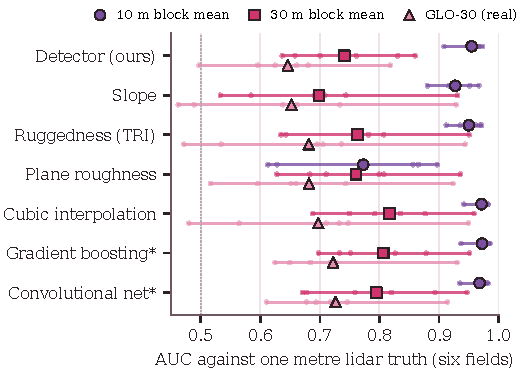
\includegraphics[width=\columnwidth]{figures/fig_auc.pdf}
\caption{Face cell detection against one metre lidar on six dune fields. Large markers: mean AUC over sites; small dots and lines: individual sites and their range. $^{*}$Trained leave one site out on lidar labels.}
\label{fig:auc}
\end{figure}

\subsection{Planning}
Table~\ref{tab:planning} and Fig.~\ref{fig:planning} give the pooled outcomes of the 600 pairs. The dune fields are hazardous: the shortest grid path crosses a face patch on 96\,\% of pairs, and the slip model alone, which avoids grades it cannot climb, still crosses one on 94\,\% of pairs at 30\,m and 85\,\% at 10\,m.

On 30\,m maps no hazard layer that a rover could compute makes routes meaningfully safer. Mission success is 6\,\% with the slip model alone and at most 11\,\% with any computable layer (interpolation, risk weighted; Holm corrected McNemar $p<0.001$). The gating policy fails in two opposite ways. The detector underestimates face prevalence, so it gates few cells: 91\,\% of pairs are routed and 92\,\% of those routes are unsafe. The learned and recalibrated layers flag so much of the dune field that most pairs cannot be routed at all (19\,\% for gradient boosting), and the few routes they find are still mostly unsafe. The real GLO-30 product gives the same picture.

On 10\,m maps every layer helps. Mission success rises from 15\,\% with the slip model alone to 24\,\% with the detector gate and 27\,\% with the detector weighting, and to 34\,\% with weighting by gradient boosting, the best computable layer (significantly above the detector with the same policy, $p<0.001$). Conservative routes with the detector are 1.17 times the straight distance. Even a perfect cell label reaches only 46\,\% at 10\,m and 59\,\% at 30\,m, because face patches below a cell's 10\,m$^2$ rule, or cut by the straight segment between two cell centres, remain. Marking every 5\,m cell that holds a face post routes all pairs and gives a mission success of 100\,\%, at 1.30 times the straight distance (Fig.~\ref{fig:map}d shows the contrast between 30\,m and 10\,m routes).

With the more pessimistic vehicle parameters of a published posterior (climbing limit 15.9 instead of 25.5\,degrees; exploratory, not registered), the gates route far fewer pairs (for example 34\,\% for the detector at 10\,m) and the ranking of the layers does not change.

\begin{table}[t]
\caption{Planning, pooled over six sites (600 pairs): unsafe share of routed pairs (U) and mission success (S), in \%. Gate: conservative policy; Weight: risk weighted policy.}
\label{tab:planning}
\centering\small
\setlength{\tabcolsep}{3.5pt}
\begin{tabular}{lcccccc}
\toprule
 & \multicolumn{2}{c}{I10} & \multicolumn{2}{c}{I30} & \multicolumn{2}{c}{G30} \\
Planner & U & S & U & S & U & S \\
\midrule
Shortest path & 96 & 4 & 96 & 4 & 96 & 4 \\
Slip model only & 85 & 15 & 94 & 6 & 95 & 5 \\
Gate: SLOPE & 79 & 17 & 88 & 3 & 98 & 0 \\
Gate: DET (ours) & 72 & 24 & 92 & 7 & 94 & 5 \\
Gate: DET-cal & 78 & 22 & 71 & 2 & 75 & 0 \\
Gate: GBM$^{*}$ & 76 & 24 & 67 & 6 & 70 & 3 \\
Gate: CNN$^{*}$ & 70 & 27 & 56 & 7 & 79 & 3 \\
Weight: DET (ours) & 73 & 27 & 93 & 7 & 94 & 6 \\
Weight: GBM$^{*}$ & 66 & 34 & 93 & 7 & 94 & 6 \\
Gate: ORACLE & 54 & 46 & 32 & 59 & 34 & 57 \\
\midrule
ORACLE-5 (5\,m) & \multicolumn{6}{c}{U 0, S 100} \\
\bottomrule
\end{tabular}
\end{table}

\begin{figure}[t]
\centering
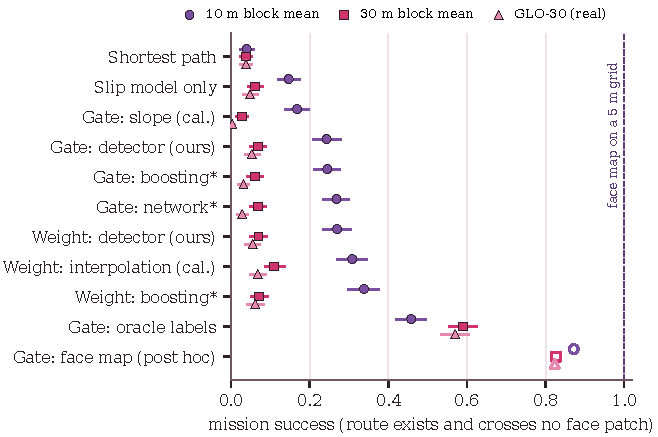
\includegraphics[width=\columnwidth]{figures/fig_planning.pdf}
\caption{Mission success of the released planner with swapped hazard layers, pooled over 600 origin and destination pairs (95\,\% bootstrap intervals). Dashed line: a 5\,m map with every face patch marked. $^{*}$Trained leave one site out on lidar labels.}
\label{fig:planning}
\end{figure}

\begin{figure*}[t]
\centering
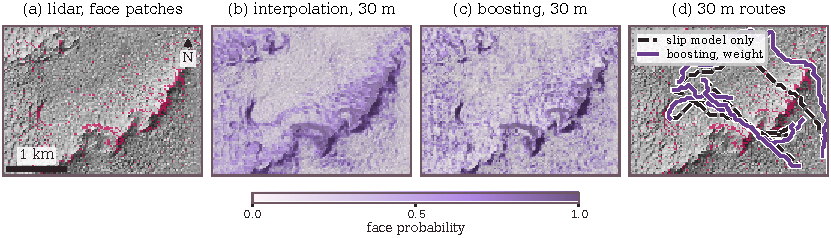
\includegraphics[width=\textwidth]{figures/fig_map.pdf}
\caption{Kelso Dunes. (a) Hillshade of the one metre lidar with face patches (pink). (b) Face probability of the detector and (c) of gradient boosting on the 30\,m block mean. (d) Conservative routes with the detector on the 30\,m map (light) and the 10\,m map (dark) over the face patches; the 30\,m routes cross faces the map cannot see.}
\label{fig:map}
\end{figure*}

\subsection{Preregistered predictions}
Of the 17 predictions registered for this benchmark, 12 were met and 5 were missed. The misses that matter for the reader are those against our own method and expectations: we expected interpolation to add nothing over slope at 30\,m (it added +0.12 mean AUC and became the best method), we expected the detector to reach an AUC of 0.93 at every site at 10\,m (it reached 0.91 at Little Sahara), and we expected the detector gate to cut the unsafe share at 10\,m by at least 15 points (it cut it by 13). The register, with every outcome and the notes written after each run, is part of the released repository.

\section{Discussion and Limitations}
\textit{What the results mean.} At 10\,m the face hazard is mostly visible and the choice of method matters little; at 30\,m it is mostly invisible and no model of the coarse surface, physical or learned, recovers enough of it to make routes safer. The strongest single cue at 30\,m is curvature: the cubic interpolation, which only exposes the curvature the coarse surface already holds, ranks face cells as well as models trained on lidar of five other fields. Our synthetic detector, trained on two dimensional straight crested profiles, ranks worse than both and underestimates how common faces are; its remaining value is that it needs no lidar and gives a probability that a recalibration on any surveyed field can correct. For a planner, the lesson is to treat a 30\,m map as a coarse prior that cannot certify ground as traversable (the released planner already refuses to call such ground verified) and to obtain a face map at about 5\,m before driving, from a drone survey, or to rely on onboard sensing.

\textit{Limitations.} The six fields are North American; the linear, star and compound megadunes of the Rub' al Khali are larger and only Great Sand Dunes holds star dunes, so the numbers transfer to Arabia as an indication only. The truth counts every surface steeper than 28\,degrees, including rock and lidar artefacts at Dumont; the secondary label limited to 36\,degrees changes little. The planning outcome is strict: any contact with a face patch of 10\,m$^2$ counts as unsafe, although some crossings would be short or survivable for a given vehicle, and a real rover would follow the route with a local planner and its own sensors. The vehicle model is an assumption range, not a measured rover, and no route was driven. GLO-30 differs from the lidar in sensor, date and datum, so the G30 results mix dune migration with product error. Six sites limit the leave one site out training of the learned baselines, and no hyperparameter was tuned for any method.

\section{Conclusion}
On six lidar dune fields, a 30\,m elevation model hides most slip faces, and neither a physically motivated detector nor models trained on lidar recover enough of them to make planned routes safer; on the real Copernicus product the loss is larger still. At 10\,m every method sees most faces and the best hazard layer more than doubles mission success over the slip model alone, but only a face map at about 5\,m makes routes safe. Map resolution, not the hazard model, is the binding constraint for small rovers on dunes. The next step is to test the same benchmark on Arabian dune fields with a drone survey and on a real rover whose slip has been measured on the same sand.

\section*{Data and Code}
USGS 3DEP lidar is in the public domain; Copernicus GLO-30 is used under its licence (produced using Copernicus WorldDEM-30 \copyright~DLR e.V. 2010-2014 and \copyright~Airbus Defence and Space GmbH 2014-2018, provided under COPERNICUS by the European Union and ESA; all rights reserved). The code, the result files, the prediction register and the scripts that regenerate every number and figure of this paper are at \url{https://github.com/hudasol/dune-rover} (stages 25 and 26).

\bibliographystyle{IEEEtran}
\bibliography{references}

\end{document}
